\scanpage{78}
\mspage{38}
Let then $\underline G'$ be a quotient MD-graph of $\underline G$ -- by a set \inserted{$C$} of edges of the graph $G$ underlying $\underline G$,
\[
(96)\qquad\underline G'=\underline G/C.
\]
We then have a \inserted{diagram of} canonical morphisms
\diagram{\begin{tikzpicture}[x=1cm,y=1cm]
\node at (-3.1,.85) {$(97)$};
\node at (0,1.8) {$\overset{\deleted{\unsure{\wedge}}}{M}_{\underline G}$};
\node at (3.0,1.9) {$\deleted{\unsure{\widehat M_{\underline G'}}}$};
\node at (0,0) {$\widehat M_{\underline G}$};
\node at (3.0,.12) {$\widehat M_{\underline G'}$};
\node at (1.48,1.80) {$\deleted{\longrightarrow}$};
\draw (.10,1.11) .. controls (.25,1.28) and (-.13,1.36) .. (-.13,1.10)
 -- (.02,.56);
\draw (3.12,1.24) .. controls (3.24,1.40) and (2.85,1.46) .. (2.87,1.20)
 -- (3.00,.65);
\draw (2.86,.82)--(3.00,.65)--(3.15,.84);
\draw (2.59,1.34)--(3.48,1.78)--(2.62,1.05)--(3.48,1.46)
 --(2.64,.73)--(3.46,1.12)--(2.70,.48);
\draw[->] (.86,.05)--(2.18,.10);
\end{tikzpicture}}
\margin{expand the definition of $\Gamma^!_{\underline G,\underline G'}$ !}
If we denote by $\Gamma^!_{\underline G,C}$ or $\Gamma^!_{\underline G,\underline G'}$ the subgroup of $\Gamma_{\underline G}$ which is formed of the automorphisms that send $C$ to itself, and that induce the identity on $\underline G'$, the \deleted{\unsure{vertical}} \inserted{horizontal} \unsure{arrow|homomorphism} $\underset{\unsure{
\begin{tikzpicture}[baseline=-.5ex,x=.10cm,y=.10cm]
\draw[line width=.4pt] (0,1)--(.8,2.3)--(1.3,2.5)--(1.0,.45)
 .. controls (.75,-.1) and (1.5,-.1) .. (1.9,.3)--(2.3,.15)--(1.7,.75);
\draw[line width=.4pt] (0,1)--(1.28,1.17)--(.70,.28)--(.38,.45)--(.82,2.30);
\end{tikzpicture}}}{\text{of}}$ (97) factors \deleted{\unsure{therefore}} \inserted{an} immersion of multiplicities
\diagram{(98):\qquad\begin{tikzcd}[ampersand replacement=\&]
(\widehat M_{\underline G},\Gamma^!_{\underline G,\underline G'})\arrow[r,hook] \& \widehat M_{\underline G'}
\end{tikzcd}}
\margin{These are perhaps only \uline{local} immersions, it seems to me -- to be checked\ldots}
I denote by $\widehat M_{\underline G,\underline G'}$ the \uline{germ of multiplicity} defined by the inclusion (98), and by $M_{\underline G,\underline G'}$ the germ defined by the induced inclusion
\diagram{(99)\qquad\begin{tikzcd}[ampersand replacement=\&]
(M_{\underline G},\Gamma^!_{G,G'})\arrow[r,hook] \& \widehat M_{\underline G'}
\end{tikzcd}}
\margin{It is better to consider the germ of multiplicity defined by the \uline{local immersion} $M_{\underline G}\longrightarrow\unsure{M_{\underline G'}|\widehat M_{\underline G'}}$, and let $\Gamma^{\unsure{!}}_{\underline G,G'}$ act on it, \unsure{and this will be} $M_{\underline G,\underline G'}$}
\margin{77}
